\documentclass[11pt]{article}
\usepackage[utf8]{inputenc}
\usepackage[T1]{fontenc} % uses T1 fonts (better quality)
\usepackage{lmodern}
\usepackage[dvipsnames]{xcolor}
\usepackage[margin=1in]{geometry}
\usepackage{graphicx} \graphicspath{ {./Images/} }
\usepackage{pdfpages}
\usepackage{booktabs}   % for table borders
\usepackage{amsmath,bm,amssymb}
\usepackage{mathtools}
\usepackage[makeroom]{cancel}
\usepackage{tikz} \usetikzlibrary{shapes,arrows}
\usepackage{wrapfig}
\usepackage{indentfirst}
\definecolor{CrispBlue}{HTML}{0176AE}
\usepackage[numbib]{tocbibind}

\begin{document}
 	\begin{center}
	\Large{\bfseries Software-Defined Networking: An Introduction to Network Softwarization}\\[1em]
	\large{David Kirby}\\
	\end{center}

\section{Abstract}

Software-defined networking can be implemented in a variety of ways, it can be centralized or distributed, it can be used in conjunction with traditional networking, or combined with NFV, network function virtualization, to support massive scale networks. For this paper, the author wishes to focus attention on the most common deployments, ones that use open source and centralized controllers. The author will be defining software-defined networking, commonly called SDN, the author will be going over the details of what has driven its evolution, and dive into the core functionalities. It is important to note that there are key advantages and disadvantages to this, and as our professor likes to say, there is no free lunch.

\section{Background}

SDN has been called, “the heart of modern networking”~\cite{Stallings}. While it is more evolutionary than revolutionary, it does bring some key functionality to networking that permits scaling of all of the topics we have been discussing over the past fifteen weeks. There are two key functions involved in forwarding packets through routers: there is a control function, which decides the route and priority the traffic will take, and a data function, which forwards data based on that control-function policy. With SDN, a central controller performs all of the complex functionality, including routing, naming, policy declaration, and security checks.\par

\begin{wrapfigure}{r}{0.2\textwidth}
	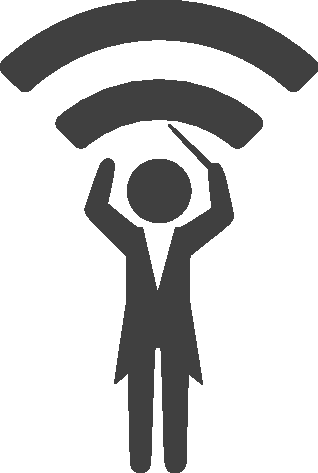
\includegraphics[width=0.2\textwidth]{NetworkConductor}
	\caption{Network Conductor}
\end{wrapfigure}

It is helpful to compare the SDN controller to an orchestra conductor. A conductor coordinates the rhythm and cadence of the musicians, rather than having each individual make their own decision about what and how they should play. Much the same way, an SDN controller coordinates network devices, determining how each device should operate.

So first, a little background on the evolving network requirements. The fourth industrial revolution is ushering in a new wave of network requirements. This demand is increasing as more devices become internet capable, as cloud services including cloud computing and cloud storage become more prevalent, and as the number of devices go from being static to being mobile~\cite{Sandberg}. Though most Internet of Thing devices are not typically bandwidth heavy, with the notable exception being surveillance video, it is the sheer number of these devices that creates a staggering load on traditional network structures.

Even as demand increases, the supply is also increasing. Bandwidth levels have grown exponentially and not only are networks tasked with serving more devices, they must do so at a much faster rate~\cite{ONF}.

Finally, traffic modes have become more complex. Traditional networks could arguably cope with the higher demand, and supply, after all, routers and switches have also advanced, but the complexity of the traffic has become more convoluted. We no longer have typical client-server models, but rather multiple servers and content distribution networks spread across large geographic areas. We have a network convergence of voice, data, and video creating unpredictable traffic patterns, along with unified communications where applications are pulling requests from multiple servers.

\section{Literature Survey}

With this evolution of network requirements, it’s important to look at the traditional network structure and determine how and if it should also evolve. Quality of Service and Quality of Experience requirements must be taken into account as one could argue that without them, the future of networking is a moot point. As with all of the previous industrial revolutions, the push for innovation is not purely for science sake, but has end users that underwrite all progress. So what is wrong with traditional networks?

Traditional networks are based on the TCP/IP architecture. As we have learned in this course, this architecture depends heavily on network interface identity, namely MAC addresses at the physical layer, and IP addresses at the network layer. Traditional networks use this addressing scheme through distributed control, that is, each router or switch has a level of autonomy where it determines the policy of the network traffic. While it is beyond the scope of this paper to go into the details of these policies, there is much more literature on these topics in~\cite{Stallings},~\cite{Sandberg}, and~\cite{Kurose}.

Routing is determined based on each packet’s destination address. In a traditional networking approach, it is possible that datagrams could be directed through different routes across the internet, as routers are constantly calculating the minimum-delay path for each packet. This optimization works great for early networks where devices are static and in a fixed location; however, there are four limitations that arise from this:

\begin{enumerate}
	\item Complexity
	\item Inconsistent policies
	\item Inability to scale
	\item Vendor dependence
\end{enumerate}

Modern networks have widely varying quality of service requirements. Traffic fluctuations and security protocols have become more complex as more devices become mobile. Supporting such massive growth with traditional networks means adding hundreds if not thousands of devices, and maintenance of such a diverse network of switches and routers is not trivial. Scaling a traditional network means rapidly adding and replacing network devices to meet demands, but this also means a wide variety of brands and models. In short, traditional networks have become a logistical nightmare for enterprises and carriers wanting to rapidly deploy new capabilities.

\section{Extended Description}

So what makes SDN a better approach? How does it solve the challenges of traditional networks? The modern approach to networking is analogous to the modern approach to computing. In the infancy of the computer age, a few vendors (namely IBM and DEC) created tightly integrated systems, designing their own proprietary compilers, processors, assembly languages, and software. This meant IBM software could not run on a DEC system. This locked users in to one system or another, and made migration to new systems extremely difficult. Modern computer systems are now able to interoperate due to a migration to open interfaces, typically running on x86 or ARM processors,  and as we see in the new Apple M1 chips, even emulation between the two can be done extremely efficiently. Designing code to run on Windows, Mac, and Linux is easier to implement based on application programming interfaces.

SDN and modern networking approaches borrow from this hardware abstraction, allowing for similar interoperability between the application layer and the network layer. This allows enterprises and carriers to tap into APIs for increased flexibility and customization. This adaptability is one of the keystones of SDN.

\begin{figure}
	\centering
	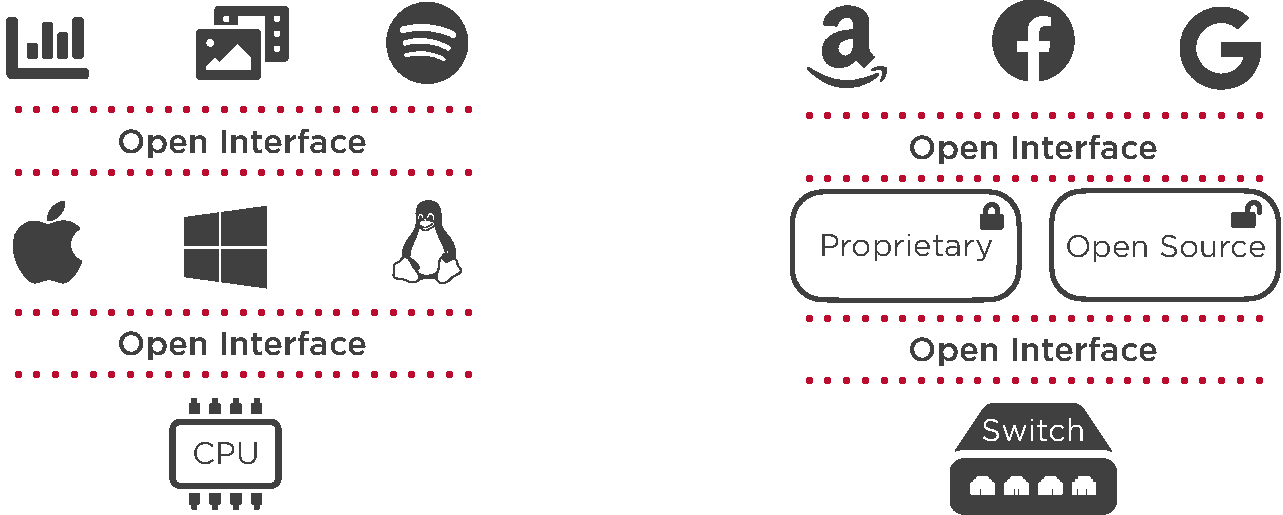
\includegraphics[width=0.75\textwidth]{ModernComparison}
	\caption[]{Modern Computing (left) and Modern Networking (right)\footnotemark\(^,\)\footnotemark}
\end{figure}
\footnotetext[1]{Adapted from \textit{Foundations of Modern Networking}~\cite{Stallings}}
\footnotetext{All trademarks, logos, and copyrights are property of their respective owners.}

SDN allows this hardware abstraction and provides a new level of customization by dividing the switching function into a data plane and a control plane, each on their own dedicated devices. Applications are able to tap into open source APIs running on top of the SDN controllers. The control plane becomes a centralized controller or set of coordinated controllers and configures the forwarding and switching tables based on this centralized view of the entire network. This allows for more dynamic provisioning of resources, best effort protocols, and security. The data plane devices become simple packet-forwarding devices. It’s important to note, however, that these data plane devices can be physical or virtual switches. This allows multiple switching devices to be run on a server via a hypervisor and with little overhead. The open nature of the SDN approach also means that SDN controllers can easily be scaled or moved to new hardware in the event of device failures.

In traditional networking, the control and data planes are combined in each switch or router and the routing functions are distributed among all of the routers of the network. Each individual knows only what it and its one-hop neighbors are doing. Using the orchestra analogy again, each musician is playing their own song, creating a cacophony of mixed protocols and routing. With modern networking, SDN controllers coordinate and fill all switching and forwarding tables in an organized and strategic manner. Resource management, protocol changes, and updates are done on the SDN controller via open source interfaces such as OpenFlow rather than being forced to update each individual router and switch.

\begin{figure}
	\centering
	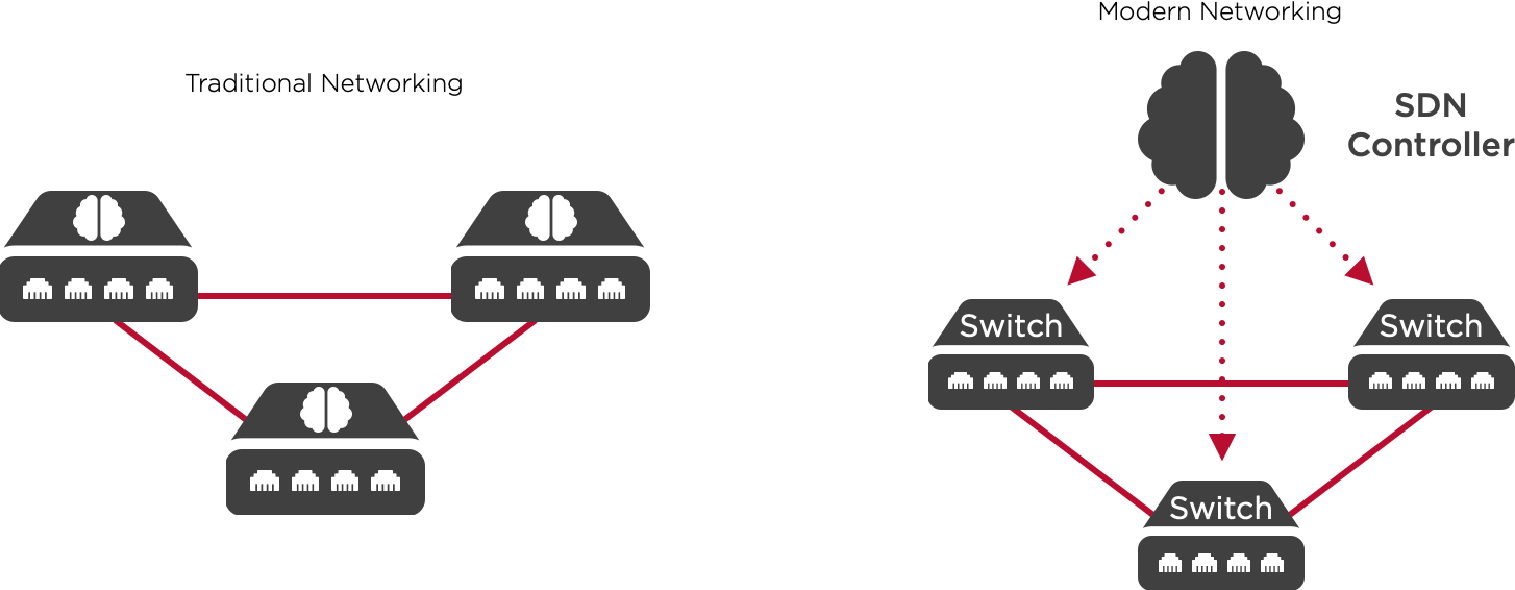
\includegraphics[width=0.8\textwidth]{SDNController}
	\caption[]{Traditional Networking (left) and Modern Networking (right)}
\end{figure}

\subsection{Data Plane}

The data plane is where network forwarding devices process all of the policies from the control plane; it is also known as the forwarding plane or infrastructure plane. This differs from traditional networking in that these devices no longer have autonomy to decide routing policies, that task has been processed by the SDN controller. The data plane continues to use forwarding tables as in traditional networks, and can adjust packet headers, place items in queue, and discard packets as we studied this semester, but now according to SDN policy.

For all of the switches and routers to behave together in accordance to the SDN policy, they must adhere to a common agreement. This adherence is based on standards and protocols that have been defined by various work groups and consortia. One such architecture is OpenFlow which runs on SDN controllers either natively installed or, most commonly, on virtual machines. These controllers then coordinate with OpenFlow-compatible switches and routers. To secure this connection, OpenFlow uses Transport Layer Security (TLS) as we discussed during this semester.

\subsubsection{OpenFlow}

OpenFlow is the most prevalent interface connecting the SDN control plane to the data plane~\cite{Coker}, but it is important to define \textit{flow}. Flow is a sequence of packets \cite{Stallings} sharing the same header fields (e.g.~sharing the same source and destination IP addresses). The OpenFlow protocol implements three types of ports: physical, which dictate the hardware interface; logical, which handle most internal connects including link-aggregation and tunnels; and reserved ports, used for non-OpenFlow connections.

\subsection{Control Plane}

In modern networking, the control plane becomes more centralized, although it can still be setup across multiple SDN controllers for redundancy, robustness, and parallelism. The control plane then takes on the following roles~\cite{Stallings}:
\begin{itemize}
	\item \textbf{Shortest path forwarding:} determines optimal path based on information from all of the network devices.
	\item \textbf{Notification management:} alarms and security state changes.
	\item \textbf{Security:} isolates and enforces application policy.
	\item \textbf{Topology:} maintains interconnections between network devices (especially virtual).
	\item \textbf{Statistics:} collects traffic data in order to better manage routing paths.
	\item \textbf{Device manager:} distributes flow tables and configures network devices.
\end{itemize}

As discussed previously, and shown in figure 2, the SDN controller is functionally similar to an operating system, allowing for network engineers to communicate with the hardware using application programming interfaces. This allows developers to design software independent of the data plane and to run on a variety of SDN controllers. One of the primary goals of SDN is to reduce vendor dependance~\cite{White}; however, this problem, while abated compared with traditional networking, remains prevalent with SDN. Open source initiatives have risen to create an open network operating systems (NOS) with which network engineers can develop software for SDN controllers. Some of these include OpenDaylight, Floodlight, Open Networking Operating System, POX, Beacon, Ryu, and Onyx. Note, however, that there are many more proprietary operating systems as shown in Figure 2, including flavors from VMWare, Nicira, and NEC~\cite{Nadeau}. Also, there are myriad ways to implement each NOS, including running variations or combinations of these proprietary and open source options, similar to how macOS is based on UNIX.

\subsubsection{OpenDaylight}

One of the most popular and widely-used network operating systems, OpenDaylight is organized by the Linux Foundation~\cite{Reza}, and as such is open source and community developed. Developers include such major players~\cite{Daylight} as Google, AT\&T, Microsoft, Verizon, Sony, and many more. Because of its support from a wide variety of industries, it is no surprise that OpenDaylight has broad use and a swath of extensions. OpenDaylight can encompass the control plane as well as parts of the application plane, allowing carriers and enterprises to develop open source software on top of the SDN controller that are highly specialized and optimized. OpenDaylight is written in Java and ran on a Java Virtual Machine (JVM), which means it can be ran on any hardware or operating system.

\begin{figure}
	\centering
	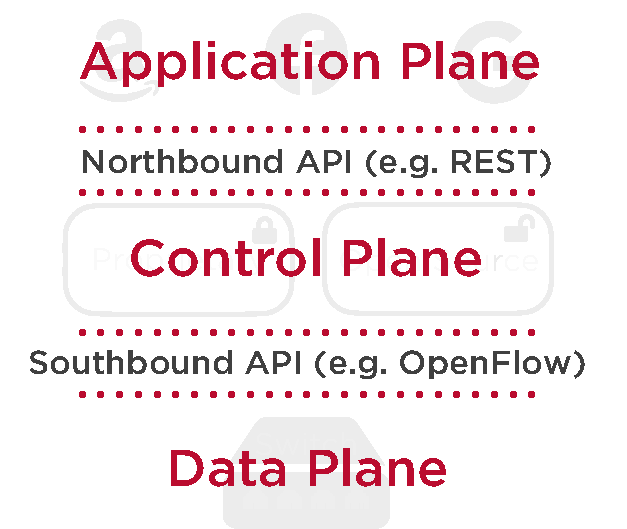
\includegraphics[width=0.4\textwidth]{Topology}
	\caption[]{Topology of Software-Defined Network}
\end{figure}

\subsubsection{REST}

We should now focus our attention on the interfaces that connect the planes of SDN,  the southbound API and the northbound API. The southbound interface we discussed with OpenFlow; it connects the data plane and the control plane. The northbound API, as the name suggests, connects the opposite direction, from the control plane up the stack to the application plane. The northbound APIs are numerous and highly focused on their particular function. One of the most common architectural styles for northbound APIs is Representational State Transfer (REST), or RESTful for styles that adhere to the REST constraints. These constraints include being client-server based, meaning it implements the request/response method; stateless, meaning the architecture does not have memory of past records, same as HTTP; cache, also like HTTP, this means that clients can be permitted to store data for later; uniform interface, this is one of the main advantages we have discussed concerning SDN; layered system, meaning the system is compartmentalized for security; and code-on-demand, meaning the API can be extended~\cite{Morreale} and to allow others features, such as allowing for Python or C++ scripts to be used.


\section{Outcomes}

Softwarization of networks allows abstraction from the hardware devices giving network engineers the ability to maintain a diverse and complex network with greater ease and flexibility. Network requirements are evolving at an exponential rate. Supply and demand are increasing, and varying traffic has created a need for more scalable and adaptable networks. Software-defined networks provide a solution by separating the control plane from the data plane, centralizing the routing functions, and implementing adaptability, automation, maintainability, model management, mobility, integrated security, and on-demand scaling~\cite{Kurose}. There is also the concern of centralization creating a single point of failure; however, this can can be mitigated by distributing the SDN control functions across multiple SDN controllers. The author would like to do much more research on how such an attack could be carried out and what methods exist to prevent such an attack. Another interesting topic the author would like to research more is the use of nested forwarding tables, ones in which tables could be subdivided based on headers. For example, dividing a flow into subflows of TCP and UDP, and further subdividing TCP into FTP, SMTP, and HTTP. The author would like to research this as a security measure and for traffic control.

\newpage

\bibliographystyle{IEEEtran}
\bibliography{final}
\end{document}